\chapter{State Of The Art} % Main chapter title

\label{Chapter2} % Change X to a consecutive number; for referencing this chapter elsewhere, use \ref{ChapterX}

%\lhead{Chapter 2. \emph{State Of The Art}} % Change X to a consecutive number; this is for the header on each page - perhaps a shortened title

%----------------------------------------------------------------------------------------
%	INTRODUCTION
%----------------------------------------------------------------------------------------

Sensor networks, as many other technological advances, see their origin on military research. They date back to the early 60's during the Cold War, when the United States deployed an underwater system to detect Soviet submarines called SOSUS (sound surveillance system). However, it is not until the beginnings of the 21st century that more applications were found beyond warfare. The main causes for that to happen is that the cost and the size of the components have drastically decreased.

Another crucial factor for this to happen is that new sets of wireless standards did see the light. On one hand we have IEEE 802.15 that allows to create low bitrate wireless networks called WPANs\footnote{Wireless personal area networks, defined in IEEE 802.15, refer to wireless networks where devices are just a few meters away from each other.} which incredibly extend battery lifetimes. On the other hand IEEE 802.11 enables wireless communications to experiment similar bitrates to those obtained in a wired network.

One of the motivations to develop an open sensor network is that normally those who are the owners of the information keep it to themselves, a situation on which nothing is given back to society. Therefore, it is important to share all gathered information.

Deploying sensor networks significantly contributes to the growth of smart cities ICT\footnote{Information and communications technology.} structures which, at the same time make social, cultural and urban development thrive\cite{caragliu2009smart}\cite{hollands2008will}.

There are already some initiatives that are based on wireless sensor networks. The word ``initiative'' is not intended to refer just to companies but also to organizations and individuals, from city halls that want to improve the daily lives of their citizens to people that want to share the environmental conditions from their balconies.

At the time of writing, we can distinguish between two main kinds of sensor networks: company-driven and community-driven networks, depending on who shapes the system.

These networks can generate a big amount of data over time, creating the necessity of storing this information somewhere. This information has to be always available for further usage. There are already some websites with the only objective of storing this information and providing useful visualization tools.

%---------------------------------------------------------------------------------------
%	SECTION 1
%----------------------------------------------------------------------------------------

\section{Company-driven sensor networks}

These kind of systems work normally in an opaque or translucent way but with the advantage that they have very clear objectives. Also, they usually have more resources, as making money is the main motivation.

Telcos have recently shown an interest for this market. Namely, in May 2013 the IMC\footnote{International M2M Council. More information is available at \url{http://www.im2mc.org}.} has seen the light, where Deutsche Telekom is the protagonist member. This organization aims to help companies adopt M2M technologies as well as making new policies concerning this branch of knowledge.

%-----------------------------------
%	SUBSECTION 1.1
%-----------------------------------
\subsection{Libelium}

Having its headquarters in Zaragoza (Spain), this is one of the biggest companies in the world built around wireless sensor networks. Libelium\footnote{\url{http://libelium.com}} offers the mechanisms and tools to deploy and build systems around the Internet of Things, smart cities and M2M\footnote{Machine-to-machine communications are established between two autonomous devices.} communications.

\begin{figure}[htbp]
    \centering
    
\includegraphics[scale=2]{./Figures/libelium_logo.png}
        \rule{35em}{0.5pt}
        \caption[Libelium logo]{Libelium logo.}
    \label{fig:ArduinoUNO}
\end{figure}

The majority of the products they sell are focused on one specific application, such as waste management, structural health, etc. These systems are intended to be bought by system integrators for end users. However, they also offer the so-called ``Waspmote'', which is a sensor device for developers that can be freely customized and reprogrammed, since it is an open hardware product. For their non-open products they provide a very complete API along with an excellent documentation.

Their products are being widely used across more than 75 countries and they are definitely one of the leaders of the wireless sensor network industry.

%----------------------------------------------------------------------------------------
%	SECTION 2
%----------------------------------------------------------------------------------------

\section{Community-led sensor networks}

Projects that are driven by the community give all the decision making power as well as resources to the community. The individuals that conform the community are very passionate about what they do and the workflow is highly transparent.

It is worth saying that the initiatives presented in this section are not sensor networks per se, but \emph{sensing networks}. This is because communication does not take place between sensor nodes but between a sensor node and a central server that processes and represents data.

%-----------------------------------
%	SUBSECTION 2.1
%-----------------------------------
\subsection{Air Quality Egg (AQE)}

This is a sensing network that aims, as its own name indicates, to measure the air quality. This is done through $NO_{2}$ and $CO$ levels.

The users are supposed to connect their ``eggs'' (or base stations) to their local network via an Ethernet inferface. Then, a bunch of outdoor sensors are placed outside and communicate their readings to the base station ---as it can be seen in figure \ref{fig:aqe}--- wirelessly through a radio frequency transmitter. Finally the data is sent in real time to Xively.

\begin{figure}[htbp]
    \centering
    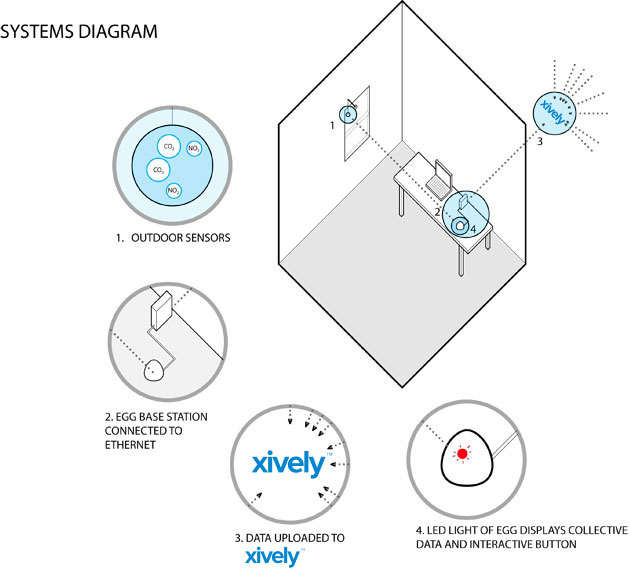
\includegraphics[scale=0.62]{./Figures/egg.jpg}
        \rule{35em}{0.5pt}
        \caption[Air Quality Egg typical scenario]{AQE typical scenario. Picture taken from the AQE official website (\url{http://airqualityegg.com})}
    \label{fig:aqe}
\end{figure}

It is worth mentioning that the AQE project is completely open, hence anyone can improve the platform as well as building his own egg from scratch without having to actually buy one.

All the information related to the hardware, software and sensor calibration can be found in their wiki\footnote{\url{http://airqualityegg.wikispaces.org}}.

%-----------------------------------
%	SUBSECTION 2.2
%-----------------------------------
\subsection{Smart Citizen}

Originally designed in Barcelona, Smart Citizen\footnote{\url{http://smartcitizen.me}} is a very young project (still in beta stage) that intends to create the biggest community around social sensing. It was initially crowdfounded in 2012 through a Goteo campaign\footnote{Goteo is a Spanish social network that helps crowdfund open projects that result in a society improvement. This campaign can still be visited at \url{http://goteo.org/project/smart-citizen-sensores-ciudadanos}} and they have succesfully launched another crowdfunding campaign on Kickstarter.

The Smart Citizen platform allows its users to precisely geolocate their data and see other users' information. There is also a very big emphasis in data sociability, since every value or datastream\footnote{Set of values that represent an individual sensor over time.} can be shared through any social networking site or inside the same web application.

Openness is as well one of their main values, since every piece of code ---including the very own website--- and hardware schematics is open source licensed.

%----------------------------------------------------------------------------------------
%	SECTION 3
%----------------------------------------------------------------------------------------

\section{Open data services}

All gathered information must be stored in some place, and this is where open data portals ---also called Internet of Things clouds--- come into play.

These websites provide users with an open API so they can upload new values, create new feeds\footnote{Representation of an environment. A feed can be, for instance, a museum hall where presence and noise levels are measured.}, retrieve the data and even create customized triggers, such as sending a push notification to a smartphone or even ``tweeting'' something. This way, we cannot only sense but \emph{react} to certain kinds of events.

Because data by itself is usually worthless, one of their most important features is the availability of data visualization tools. They allow us to easily detect patterns and also correlate certain factors.

Good examples of these sites are, as mentioned before, Xively and Sen.se\footnote{\url{http://open.sen.se/}}. Pompeu Fabra University has its own cloud to store sensory data as well, called Open Sensor Network Web Application\footnote{Available at \url{http://opencities.net/}.}. All these options are free to use and very easy to interact with, since they provide us with a RESTful API\footnote{Web API that works with the regular HTTP methods. That is, \texttt{GET}, \texttt{PUT}, \texttt{POST} and \texttt{DELETE}.}.

In case we want to host our own cloud for the Internet of Things, there is also a great solution called Nimbits\footnote{\url{http://nimbits.com}}. It is open source software and anyone can install it in its own server.
